\documentclass[letterpaper,12pt]{article} % Documento en dos columnas, tamaño carta
\usepackage[spanish]{babel}       % Traduce capítulos, fechas, etc. al español
\usepackage[utf8]{inputenc}       % Permite usar acentos directamente
\usepackage[T1]{fontenc}          % Codificación para que se vean bien los caracteres en PDF
\usepackage{lmodern}              % Usa fuentes escalables compatibles con microtype
\usepackage{geometry}             % Control de márgenes y tamaño de página
\usepackage{fancyhdr}            % Encabezados y pies de página personalizados


%Notación 

\usepackage{amsmath}  % Ecuaciones, símbolos y fuentes matemáticas
\usepackage{amssymb}
\usepackage{amsfonts}
\usepackage{siunitx}                     % Escritura coherente de unidades del SI y números

%gráficos 

\usepackage{graphicx}           % Insertar y escalar imágenes
\usepackage{subcaption}         % Subfiguras dentro de una figura
\usepackage{booktabs}           % Tablas más profesionales
\usepackage{longtable}          % Tablas que ocupan varias páginas
\usepackage{tabularx}           % Tablas con ancho ajustable automáticamente
\usepackage{array}              % Mejoras en tablas y alineación de columnas
\usepackage{float}              % Control de posición de figuras y tablas


% --- COLORES Y LISTAS PERSONALIZADAS ---
\usepackage{xcolor}             % Uso de colores en texto y figuras
\usepackage{enumitem}           % Listas personalizadas (espaciado, numeración)

% --- HIPERVÍNCULOS Y NAVEGACIÓN ---
\usepackage[hidelinks]{hyperref}           % Enlaces ciclables en PDF (índice, URLs, referencias)
\usepackage{biblatex}           % Gestión de bibliografía (citas, referencias)

% --- DIAGRAMAS TÉCNICOS ---
\usepackage{tikz}                         % Gráficos vectoriales (bloques, flujos, redes)
\usepackage{forest}                      % Árboles, jerarquías (estructuras)

% --- ALGORITMOS Y CÓDIGO FUENTE ---
\usepackage{algorithm2e}    % Pseudocódigo paso a paso (algoritmos)
\usepackage{listings}       % Mostrar código fuente con formato

\geometry{letterpaper, margin=1in} % Márgenes de 1 pul
\title{Ayahuik 1: Guía de Misión}
\author{CUAUHTÉMOC IPN}


\pagestyle{fancy} 
\setlength{\headheight}{14.5pt}
\fancyhf{}
\fancyhead[C]{Cuauhtemoc IPN}
\fancyhead[R]{AYAHUIK 1}
\fancyhead[L]{Guia de Misión}
\fancyfoot[R]{\thepage}

\graphicspath{{Imagenes/}}

\begin{document}

\tableofcontents


\newpage
\section{Antecedentes}

    \subsection{Antecedentes Históricos}

    \subsection{Antecedentes IPN}

    \subsection{Antecedentes Cuauhtémoc IPN}

    \newpage

\section{Descripción general de la misión}

    \subsection{Participantes de la misión}

    La misión Ayahuik 1 es una misión de alto impacto del equipo Cuauhtémoc IPN, la cual tendra
    participacion de varios estudiantes de diferentes unidades academicas del IPN, incluidas ESIME Ticoman, 
    ESIME Culhuacan, ESIME Zacatenco, UPIITA, ESCOM, ESIQUIE entre otras, asi como profesores asesores de las mismas 
    unidades academicas.

    \subsection{CONOPS}

    A partir de de las simulaciones con las fechas y horas establecidas se procedera a:

    \medskip   \qquad Se llenara el globo de helio hasta superar su punto de flotabilidad neutra.

    \medskip   \qquad Se iniciaran los sistemas de la carga util.

    \medskip   \qquad Se iniciara la cuenta regresiva para la liberacion del globo.
    
    \vspace{5mm}

    Se liberara el globo sonda y se iniciara el vuelo.

    \medskip   \qquad Se iniciara la recolección de datos de telemetría.

    \medskip   \qquad Se debera realizar monitoreo constante del vuelo.

    \medskip   \qquad Una vez alcnaza la altitud objetibo se debera reventar el globo sonda.

    \medskip   \qquad Se debera realizar el rastreo contante en el descenso.
    
    \vspace{5mm}

    Una vez que la carga util toque tierra se debera proceder a su recuperacion.

    \medskip   \qquad Se debera proceder a la recuperacion de la carga util.

    \medskip   \qquad Se debera asegurar tanto camaras como datos almacenados.

    \subsection{Descripción de la carga util}

    La carga util debera esta rconstituida por una plataforma en la cual debera tener 
    la capacidad de resistir las condiciones adversas de la estratosfera, asi como la obtencion
    de los siguientes datos:

    \begin{itemize}
        \item Temperatura, humedad, altitud, aptitud, velocidad, rayos ultravioleta.
        \item Gases atmosfericos (Oxigeno, hitrogeno, nitrogeno).
        \item Gases vulcanicos (Dióxido de carbono, Dióxido de azufre).
        \item Posicionamiento GNSS.
        \item Estacion meteorológica.
        \item Radio baliza.
        \item Radio localizador.
        \item Camaras de video y fotografía.
        \item ETC. 
    \end{itemize}

    \subsection{Descripción del proceso de diseño y construcción}

    \subsection{Descripción del lanzamiento y recuperación}

    Al momento del lanzamiento del globo sonda, este debera contar con analisis previos
    de trayectoria ya que la cuenca del valle de Mexico y las zonas cercanas contienen rutas
    aereas de gran importancia del pais asi como la cercania de varios aeropueros los cuales 
    son el aeropuero Marino Matamoros, aeropuero Internacional de Toluca, Aeropueto internacionl de Prueba, Aeropuerto Nacional Mexiquense “Dr. Jorge Jiménez Cantú”
    y el mas importante el Aeropuerto Internacional de la Ciudad de México el cual es el
    mas importante del país, por lo cual se debe contar con un plan de vuelo y una trayectoria 
    que evite zonas restringidas nacionales e internacionales, así como evitar rutas aereas de gran importancia.
    Por lo mismo se debera contar con los permisos necesarios por parte de la Direccion General de Aeronautica Civil,
    Agencia Federal de Aviación Civil para el lanzmaiento del globo sonda.

    \begin{figure}[H]
      \centerline{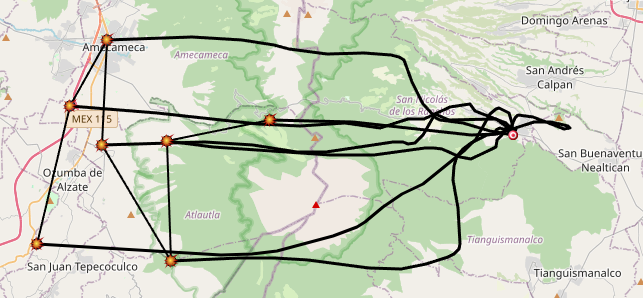
\includegraphics[width=1\textwidth]{Tray.png}}
      \caption{Trayectorias estimadas para el mes de Julio}
      \label{fig:Trayectoria}
    \end{figure}

    \begin{figure}[H]
      \centerline{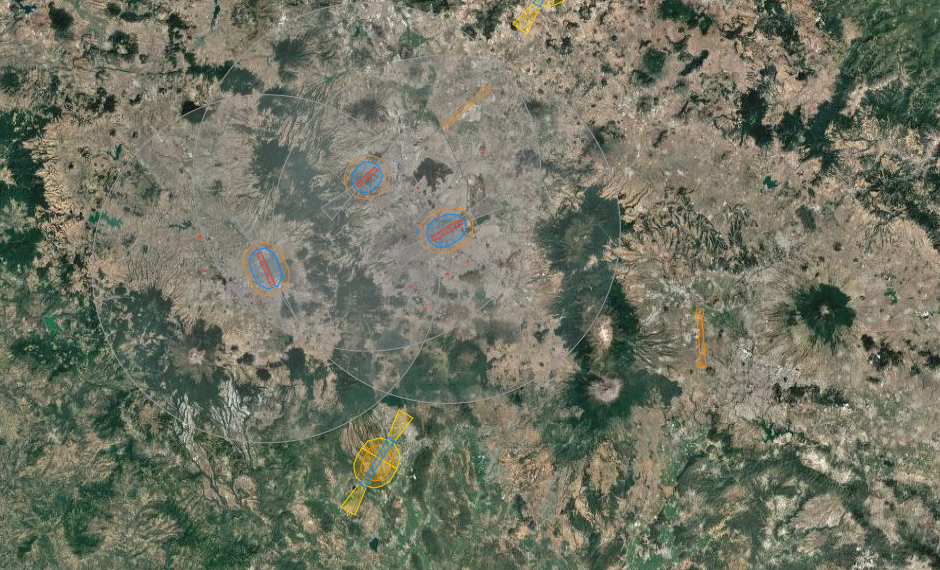
\includegraphics[width=.8\textwidth]{Zonas.png}}
      \caption{Zonas con restricciones aereas cercanas}
      \label{fig:Zonas}
    \end{figure}

    \begin{figure}[H]
      \centerline{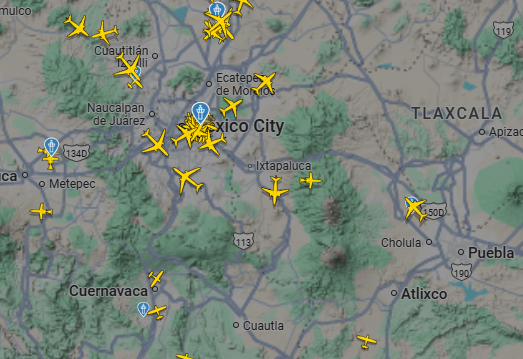
\includegraphics[width=.8\textwidth]{Espacioaereo.png}}
      \caption{Espacio y transito aereo sobre el valle de la ciudad de Mexico}
      \label{fig:Espacio}
    \end{figure}

    Se debera realizar un analisis exhaustivo en conjunto de las autoridades mexicanas 
    para decidir el mejor dia y hora del lanzamiento del globo sonda, la zona de recuperación se 
    establecera en varios puntos a partir de las simulaciones de trayectoria y el viento, asi como 
    la trayectoria qeu siga el globo al momento del vuelo.


\newpage
\section{Objetivos y criterios de éxito}

    \subsection{Objetivos generales}
    La misión Ayahuik 1 tiene como objetivo principal el desarrollo de una carga util capaz de ser lanzada a la estratosfera
    y recuperar parámetros atmosféricos y de condiciones del aire a diferentes alturas,
    así como la obtención de material fotográfico y de video del lanzamiento y vuelo de la misma.


    Esto con el fin de la obtención de datos científicos como de divulgación.

    \subsection{Objetivos específicos}
    \begin{itemize}
        \item El desarrollo de una carga util de un globo sonda la cual demuestre las capacidades desarrollo tecnológico de los miembros del equipo Cuauhtémoc IPN.
        \item Fotografía y video de las zonas aledañas al volcán Popocatepetl.
        \item Sondeo de gases en diferentes altitudes en las zonas aledañas al volcán Popocatepetl.
        \item Recolección de datos atmosféricos y de condiciones del aire a diferentes alturas
        \item Capacitación de las nuevas generaciones del equipo tanto en ámbitos tecnológicos como de documentación y divulgación.
        \item Incentivación del desarrollo de nuevas tecnologías y retos para los miembros del equipo.
        \item Divulgación científica con los datos y videos obtenidos al vuelo.
        
    \end{itemize}    

    \newpage
    
    \subsection{Criterios de éxito}

    Los criterios de éxito de la misión se basaran en una ponderación al 100\% de los hitos obtenidos durante el desarrollo de la misión en su etapa de vuelo dependiendo de su importancia y complejidad los cuales son desarrollados a continuación:

    \begin{longtable}{|m{4.1cm}|c|c|c|}
    \hline
    \textbf{Criterio de Éxito} & \textbf{Puntos máximos} & \textbf{Puntos Obtenidos} & \textbf{Observaciones} \\
    \hline
    \endfirsthead
    \hline
    \textbf{Criterio de Éxito} & \textbf{Puntos máximos} & \textbf{Puntos Obtenidos} & \textbf{Observaciones} \\
    \hline
    \endhead
    Vuelo a grandes altitudes & 10 &  & \\
    \midrule
    Medición de temperatura en vuelo & 10 &  & \\
    \midrule
    Medición de la presión en vuelo & 10 &  & \\
    \midrule
    Medición de oxigeno en vuelo & 10 &  & \\
    \midrule
    Medición de vapor de agua en vuelo & 10 &  & \\
    \midrule
    Medición del gas $H_{2}$ en vuelo & 10 &  & \\
    \midrule
    Medición del gas $CO_{2}$ en vuelo & 10 &  & \\
    \midrule
    Medición del gas $SO_{2}$ en vuelo & 10 &  & \\
    \midrule
    Toma de fotografía del Popocatepetl & 10 &  & \\
    \midrule
    Toma de video del Popocatepetl & 10 &  & \\
    \midrule
    Toma de fotografía del horizonte & 10 &  & \\
    \midrule
    Toma de video del horizonte & 10 &  & \\
    \midrule
    Recepción de telemetria por RF & 10 &  & \\
    \midrule
    Recepción de telemetria por SMS & 10 &  & \\
    \midrule
    Recepción de telemetria por MSM & 10 &  & \\
    \midrule
    Señal GNSS constante & 10 &  & \\
    \midrule
    Recuperación total de la carga util & 10 &  & \\
    \midrule
    Estado de la carga util al recuperar & 10 &  & \\
    \midrule
    Control autónomo en la etapa de descenso & 10 & & \\
    \midrule
    Funcionamiento de la Estación Terrena & 10 &  & \\
    \midrule
    Funcionamiento de la computadora de vuelo & 10 &  & \\
    \midrule
    Funcionamiento de la electronica & 10 &  & \\
    \midrule
    \textbf{TOTAL} & 220 &  & -\\
    \hline
    \end{longtable}

    Por lo tanto el porcentaje de Éxito de la misión es de: $\%$

    Éxito mínimo < 50\%

    Éxito parcial 50\% - 80\%

    Éxito total 80\% - 100\%

    \newpage

    \subsection{Restricciones y requerimientos}

    \begin{longtable}{|l|m{15cm}|}
    \hline
    \textbf{No.} & \textbf{Restricción/Requerimiento} \\
    \hline
    \endfirsthead
    \hline
    \textbf{No.} & \textbf{Restricción/Requerimiento} \\
    \hline
    \endhead
    1 & La masa total de la carga útil no debe exceder 1 kg. \\
    \midrule
    2 & La carga util debe ser capaz de soportar las adversas condiciones de 20 km de altitud. \\
    \midrule
    3 & Se debe contar con una reserva energética de al menos el $100\%$ de la misión. \\
    \midrule
    4 & Ningún elemento debe sobresalir del area delimitada para la carga util. \\
    \midrule
    5 & La carga util deberá ser capaz de decender al momento del toque de tierra a 5 m/s verticales. \\
    \midrule
    6 & La carga util deberá estar hecha de colores fosforescentes o reflectantes para su localización. \\
    \midrule
    7 & No se debe usar pirotecnia. \\
    \midrule
    8 & Se debe logar la recolección de todos los datos de vuelo. \\
    \midrule
    9 & Se debe contar con un sistema de GNSS o a través de triangulación por RF. \\
    \midrule
    10 & La telemetria se debe almacenar en una memoria interna. \\
    \midrule
    11 & La telemetria debe ser expuesta en uns estación terrena.   \\
    \midrule
    12 & La telemetria también debe ser enviada por SMS Y MSM. \\
    \midrule
    13 & La carga util debe estar identificada con el nombre del equipo asi como un medio de contacto. \\
    \midrule
    14 & Debe haber un interruptor de apagado y encendido del modelo. \\
    \midrule
    15 & Se debe contar con un sistema de audio beacon para la localización en tierra. \\
    \midrule
    16 & Se debe contar con al menos 2 sistemas de explosion o liberación de emergencia del globo.    \\
    \midrule
    17 & Se debe contar con una radiobaliza \\
    \hline
        
    \end{longtable}

    \newpage
\section{Resultados esperados}

    La misión contara con diferentes resultados esperados, los cuales se dividen en resultados técnicos, de la carga util y de la misión en general, 
    los cuales validaran el correcto desarrollo y éxito total o parcial de la misión.

    \subsection{Resultados técnicos}

    documentación técnica de la carga util y sistemas asi como del desarrollo de los mismos
    (PDR, CDR y PFR).
    Asimismo un documento con los resultados de las pruebas ambientales realizadas (vació, térmica, vibraciones y drop test)
    detallando el desempeño de la carga util y validando a la misma para su lanzamiento. 

    \subsection{Resultados de la carga útil}

    Carga util reutilizable que cumpla con todos los requisitos establecidos para la misión, la cual
    demuestre tener capacidades de recolección de datos y transmisión de los mismos tanto por radio
    frecuencia como por SMS y MSM a una estación terrena.
    
    Esta deberá contar con manual de operaciones 
    para la correcta operación y recuperación de la carga util.
    
    La misma deberá ser capaz de resistir las condiciones de lanzamiento y vuelo con condiciones extremas de presión y temperatura,
    asi como de ser capaz de soportar el retorno a tierra y ser recuperada en condiciones de operatividad.


    \subsection{Resultados de la misión}

    Obtención de datos atmosféricos y de condiciones del aire a diferentes alturas de gran utilidad
    científica y de investigación, asi como material fotográfico y de video del lanzamiento y vuelo desde la carga util.
    
    Aprendizaje y capacitación practica para la nueva generación del equipo Cuauhtémoc IPN 2025-2026 a lo largo de diferentes
    ámbitos tanto de desarrollo técnico como de generación de documentación técnica y de gestión de proyectos de alto impacto. 



\newpage

\section{Organización del equipo}

    El equipo Cuauhtémoc IPN está organizado en diferentes subsecciones para asegurar el funcionamiento del equipo y una gestión 
    eficiente de las misión, todas estas serán coordinadas por los líderes de misión 
    y estos a su ves por los capitanes del equipo. 
    \begin{figure}[!h]
      \centerline{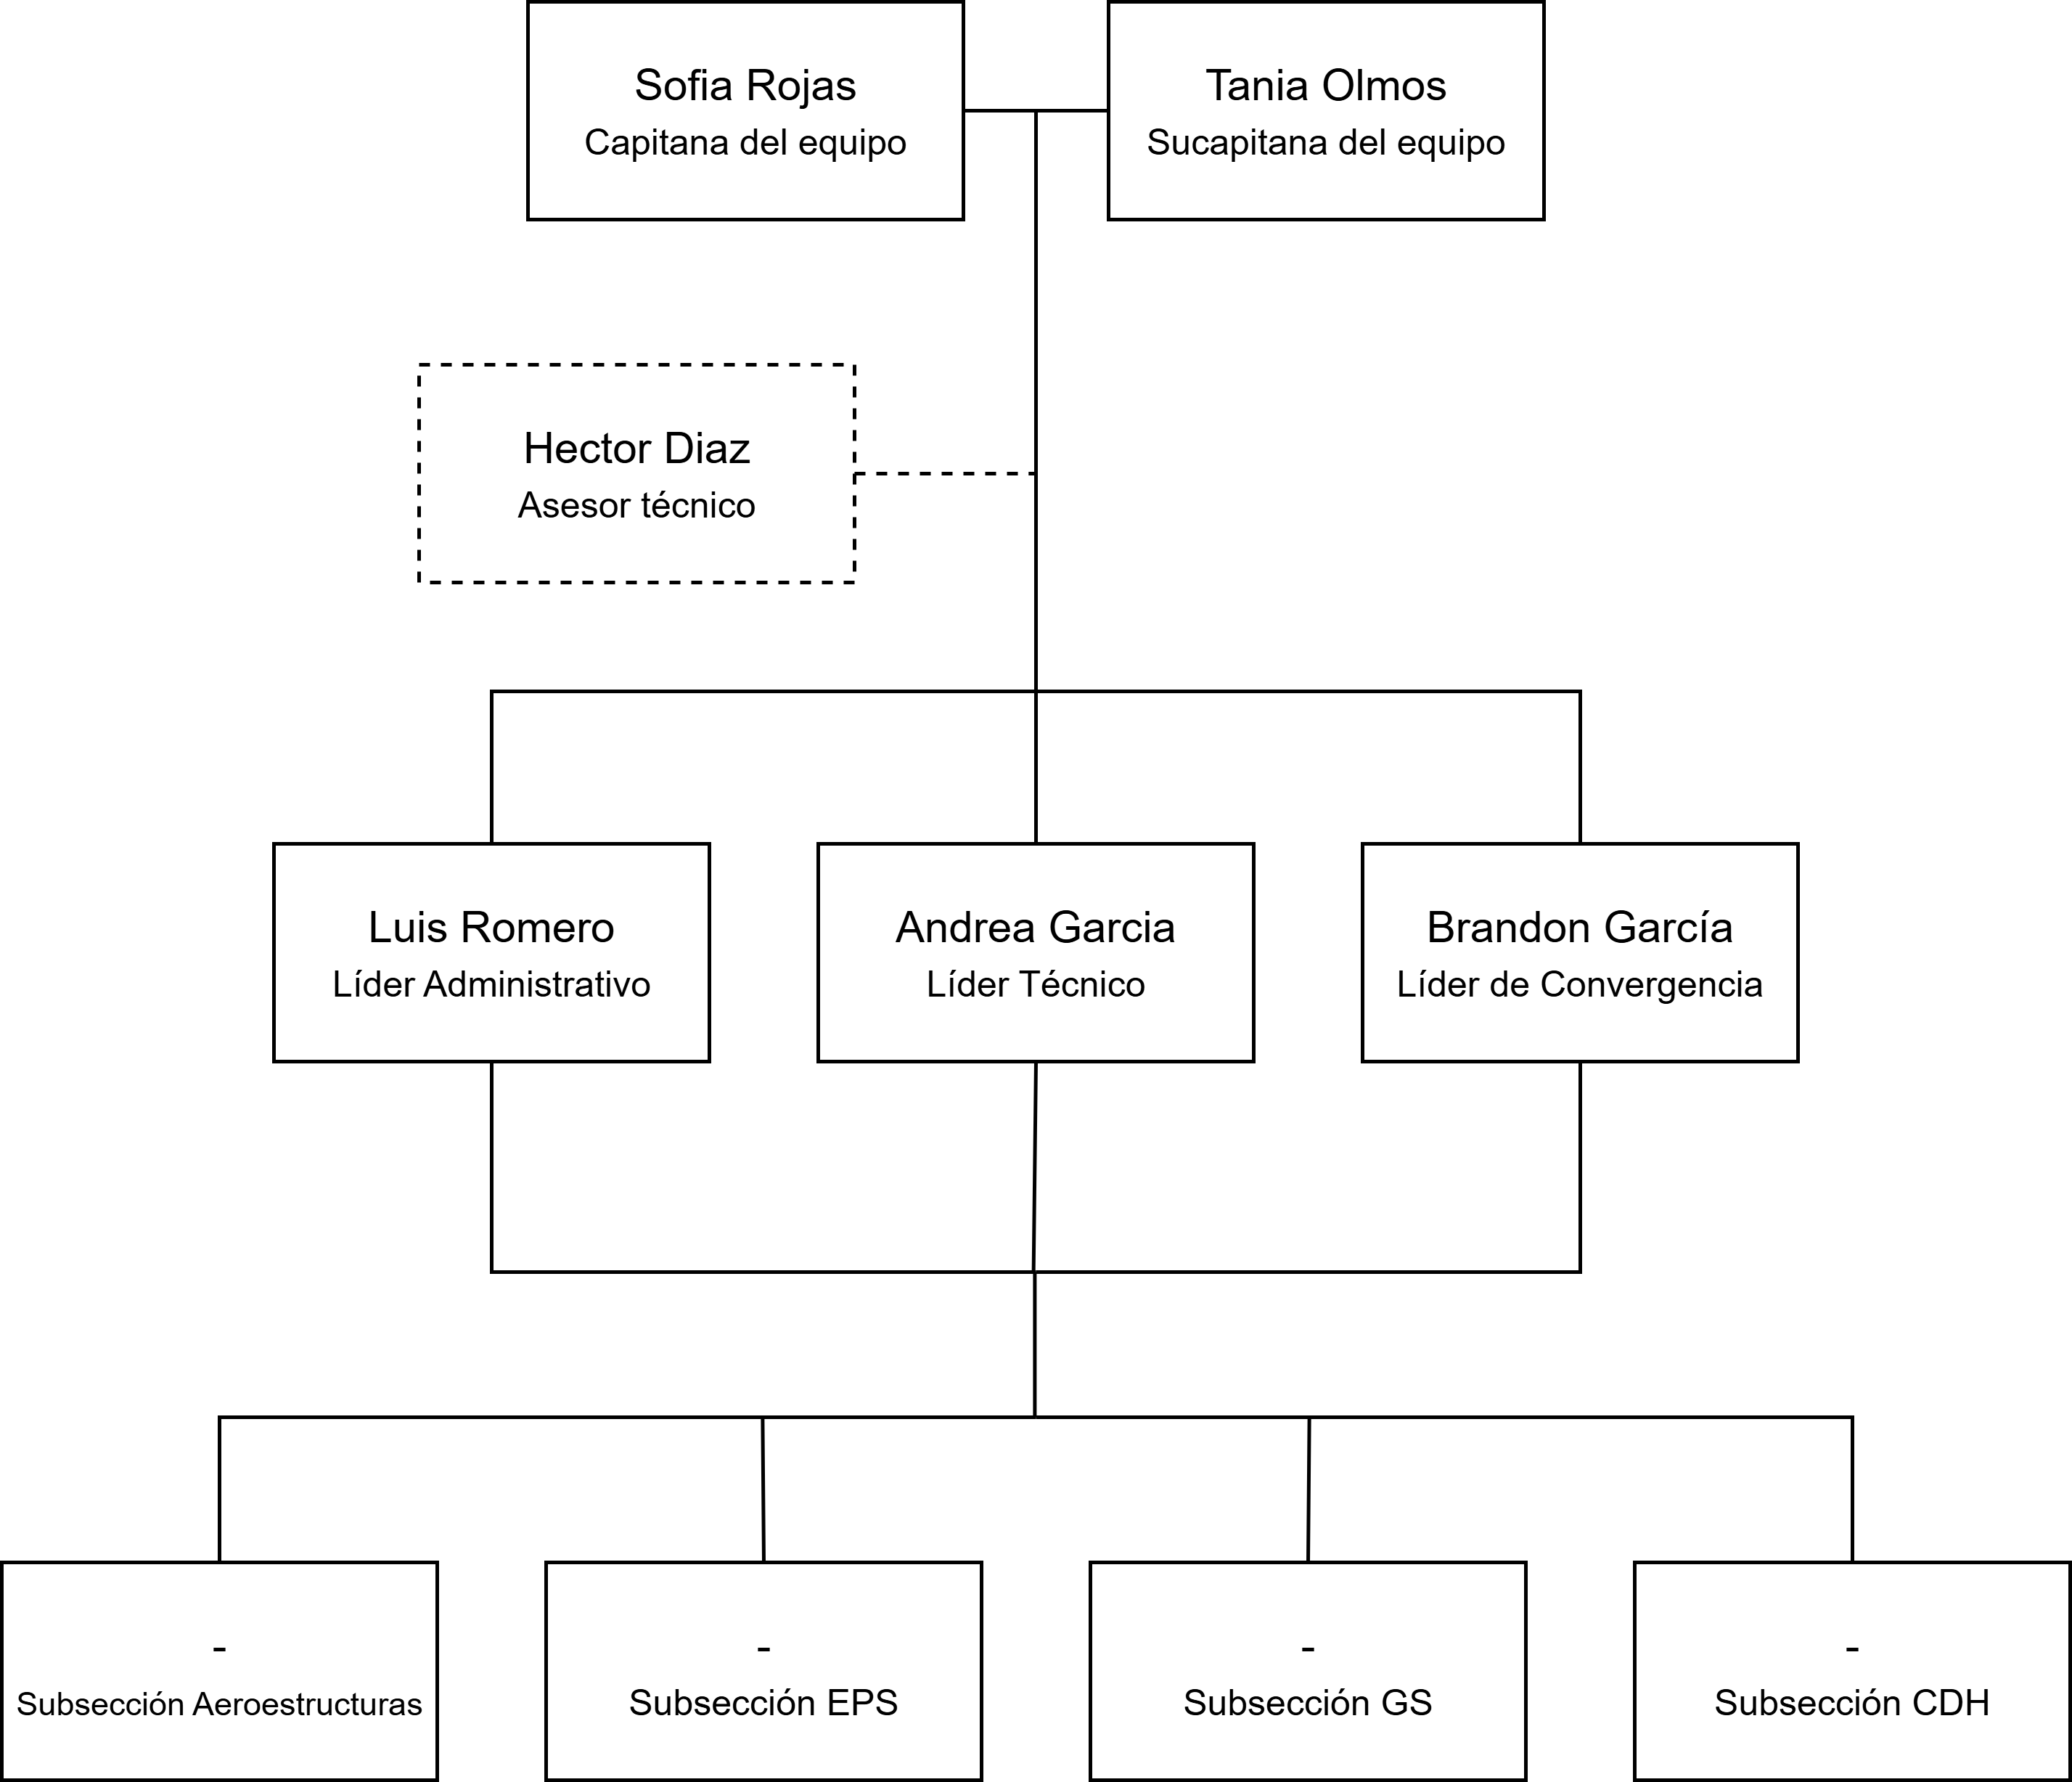
\includegraphics[width=.8\textwidth]{ORG-AYA1-GM-V3.png}}
      \caption{Organigrama Ayahuik 1}
      \label{1}
    \end{figure}
    
    Para la misión Ayahuik 1, el equipo Cuauhtémoc IPN contara con las 2 capitanas del equipo, 
    las cuales se encargaran de coordinar las actividades generales del equipo asi como sus misiones activas, 
    estas son:

    \begin{itemize}
        \item \textbf{Capitana:} Sofia Rojas
        \item \textbf{Subcapitana:} Tania Olmos
    
    \end{itemize}

    De esto se derivara el asesor técnico el cual se encargara de todo el asesoramiento tanto para el funcionamiento del equipo
    como para la correcta realización de la misión sin que este tenga intervención directa, el cual es:

    \begin{itemize}
        \item \textbf{Asesor técnico:} Hector Diaz

    \end{itemize}


    \vspace{5mm}

    El liderato de la misión AYAHUIK 1 estará a cargo de 3 co-líderes,
    los cuales se encargaran de coordinar el correcto funcionamiento de Cada
    una de las subsecciones del equipo, estos son:

    \begin{itemize}
        \item \textbf{Líder administrativo:} Luis Romero
        \item \textbf{Líder técnico:} Andrea Garcia
        \item \textbf{Líder de convergencia:} Brandon Garcia
    
    \end{itemize}

    De los cuales se derivaran las subsecciones del equipo, las cuales son aeroestructuras, EPS (Electrical Power System), GS (Ground Station) y CDH (Communication and Data Handling).

    \newpage

\section{Bibliografía}
    \begin{thebibliography}{9}
        \bibitem{NASA} NASA. (2023). High Altitude Ballooning. Recuperado de \url{https://www.nasa.gov/ballooning}
        \bibitem{ESA} ESA. (2023). Stratospheric Balloon Missions. Recuperado de \url{https://www.esa.int/stratospheric_ballooning}
        \bibitem{IPN} Instituto Politécnico Nacional. (2023). Cuauhtémoc IPN. Recuperado de \url{https://cuauhtemoc.ipn.mx}
        \bibitem{ESIME} ESIME Ticoman. (2023). Proyectos de investigación y desarrollo tecnológico. Recuperado de \url{https://esime-ticoman.ipn.mx/proyectos}

    \end{thebibliography}

    \section{Patrocinadores}
    \captionsetup[subfigure]{labelformat=empty}

    \begin{figure}[h!]
    \centering
    \begin{subfigure}[b]{0.3\textwidth}
        \centering
        
\includegraphics[height=3cm]{IPN.png}
        \caption{IPN}
        \label{fig:IPN}
    \end{subfigure}
    \hfill
    \begin{subfigure}[b]{0.3\textwidth}
        \centering
        
\includegraphics[height=3cm]{ESIME.png}
        \caption{ESIME Ticoman}
        \label{fig:ESIME}
    \end{subfigure}
    \hfill
    \begin{subfigure}[b]{0.3\textwidth}
        \centering
        
\includegraphics[height=1.8cm]{FUNDPOL.png}
        \vspace{0.5cm}
        \caption{Fundación Politécnico}
        \label{fig:FUNDPOL}
    \end{subfigure}
    \end{figure}


    \begin{figure}[h!]
    \centering
    \begin{subfigure}[b]{0.3\textwidth}
        \centering
        
\includegraphics[height=2cm]{ALTIUM.png}
        \caption{ALTIUM}
        \label{fig:ALTIUM}
    \end{subfigure}
    \hfill
    \begin{subfigure}[b]{0.3\textwidth}
        \centering
        
\includegraphics[height=1cm]{ALTAIR.png}
        \vspace{0.1cm}
        \caption{ALTAIR}
        \label{fig:ALTAIR}
    \end{subfigure}
    \hfill
    \begin{subfigure}[b]{0.3\textwidth}
        \centering
        
\includegraphics[height=1.2cm]{PCBMEX.png}
        \vspace{0.5cm}
        \caption{PCB México}
        \label{fig:PCBMEX}
    \end{subfigure}
    \end{figure}

    \hspace{0.3cm}
    \begin{figure}[h!]
    \centering
    \begin{subfigure}[b]{0.3\textwidth}
        \centering
        
\includegraphics[height=1.1cm]{SSC.png}
        \vspace{0.2cm}
        \caption{GRUPO SSC}
        \label{fig:SSC}
    \end{subfigure}
    \hfill
    \begin{subfigure}[b]{0.3\textwidth}
        \centering
        
\includegraphics[height=1.5cm]{ANSYS.png}
        \caption{ANSYS}
        \label{fig:ANSYS}
    \end{subfigure}
    \hfill
    \begin{subfigure}[b]{0.3\textwidth}
        \centering
        
\includegraphics[height=1.2cm]{DASSAULT.png}
        \vspace{0.2cm}
        \caption{DASSAULT SYSTEMES}
        \label{fig:DASSAULT}
    \end{subfigure}
    \end{figure}
    
    \hfill


    Gracias por su apoyo, sin ustedes nada de esto sería posible.

    Atte. Cuauhtémoc IPN

    \end{document}
